\documentclass[a4paper,12pt]{scrartcl}

\newcommand{\dropsign}[1]{\smash{\llap{\raisebox{-.5\normalbaselineskip}{$#1$\hspace{2\arraycolsep}}}}}%

\usepackage[utf8]{inputenc}
\usepackage[ngerman]{babel}
\usepackage{multicol}
\usepackage{scrpage2}\pagestyle{scrheadings}
\usepackage{graphicx} 

\ihead{Blatt 2, G2B}
\chead{Elena Noll, Sven-Hendrik Haase, E. Böhmecke}
\ohead{\today}
\pagestyle{scrheadings}
\setheadsepline{1pt}
\setcounter{secnumdepth}{0}

\begin{document}

\section{Aufgabe 6}
\subsection{a)}
Ja, der Code C\textsubscript{1} erfüllt die Präfixbedingung. Keines der Codewörter ist Beginn eines anderen Codewortes.
\\\\
Diese Anforderung ist wichtig beim auslesen von mehreren Codewörtern. Wenn wir auf ein Codewort treffen können wir sofort zum nächsten Wort  übergehen da wir wissen, dass kein anderes Wort mit dem gefundenen Codewort anfängt.

\subsection{b)}
\begin{displaymath}
L(C) = (1*\frac{2} {5})+(3*\frac{2} {15})+(3*\frac{1} {5})+(2*\frac{4} {15})
\end{displaymath}
\begin{displaymath}
L(C) = \frac{2} {5} + \frac{2} {5} + \frac{3} {5} + \frac{8} {15}
\end{displaymath}
\begin{displaymath}
L(C) = 1,9\overline{3}
\end{displaymath}
\\\\
\begin{displaymath}
h = (\frac{2} {15}*2,907)+(\frac{1} {5}*2,322)+(\frac{4} {15}*1,907)+(\frac{2} {5}*1,322)
\end{displaymath}
\begin{displaymath}
h = 1,89
\end{displaymath}
\\\\
\begin{displaymath}
R\textsubscript{Code} = L(C) - h
\end{displaymath}
\begin{displaymath}
R\textsubscript{Code} = 1,93 - 1,89
\end{displaymath}
\begin{displaymath}
R\textsubscript{Code} = 0,04
\end{displaymath}
\subsection{c)}
\begin{displaymath}
L(C) = (2*\frac{2} {5})+(2*\frac{2} {15})+(2*\frac{1} {5})+(2*\frac{4} {15})
\end{displaymath}
\begin{displaymath}
L(C) = \frac{4} {5} + \frac{4} {15} + \frac{2} {5} + \frac{8} {15}
\end{displaymath}
\begin{displaymath}
L(C) = 2
\end{displaymath}
\\\\
\begin{displaymath}
h = (\frac{2} {15}*2,907)+(\frac{1} {5}*2,322)+(\frac{4} {15}*1,907)+(\frac{2} {5}*1,322)
\end{displaymath}
\begin{displaymath}
h = 1,89
\end{displaymath}
\\\\
\begin{displaymath}
R\textsubscript{Code} = L(C) - h
\end{displaymath}
\begin{displaymath}
R\textsubscript{Code} = 2 - 1,89
\end{displaymath}
\begin{displaymath}
R\textsubscript{Code} = 0,11
\end{displaymath}

\subsection{d)}
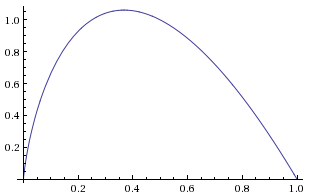
\includegraphics{./images/Aufgabe6d}

\subsection{e)}
Ja, denn ein Code kann nur ein Präfix eines anderen Codes sein wenn es kurzer ist.

\subsection{f)}
C = \{''A'', ''B'', ''C''\}\\
Quellencodierung C\textsubscript{1} ist ''A'' $\rightarrow$ 0, ''B' $\rightarrow$ 1, ''C' $\rightarrow$' 01\\\\
Wenn wir jetzt Bitfolge ''01'' betrachten könnte man entweder das Wort ''AB'' lesen oder das Wort ''C''.

\section{Aufgabe 7}
\subsection{a)}
h\textsubscript{c} = min \{h (U, U‘) $\vert$ U, U‘ $\in$ U\textsubscript{c} $\wedge$ U $\not=$ U‘\}

\subsection{b)}
Der Hemmingabstand des Codes C ist 3, da der kleinste Abstand zwischen den Codewörtern 3 ist. \\\\
Die Bitfehler die bei der Übertragung der unter Nutzung von C codierten Zeichen Z\textsubscript{1},Z\textsubscript{2},Z\textsubscript{3},Z\textsubscript{4} noch zuverlässig erkannt werden können ist: h-1 Bitfehler, also bis zu $\leq$2 Bitfehler.\\\\
Nein es spielt keine Rolle denn der Hemmingabstand ändert sich dadurch nicht.

\subsection{c)}
Dieser Code gestattet eine Fehlerkorrektur von bis zu x*3 Bitfehlern. (Herleitung aus der Formel: 2*d+1 $\rightarrow$ Korrektur aller v-Bit-Fehler, v $\leq$ d, v $\in$ N)\\\\
Dieser Fehlerkorrektur ist allerdings nicht zuverlässig. Es bleibt das Risiko einer fehlerhaften ''Korrektur''.

\section{Aufgabe 8}
\subsection{c)}
Unsere zu verschickende Nachricht $\rightarrow$ 1001011101\\\\
Als erstes wandeln wir unser Generatorpolynom in eine Bitfolge um:\\
$x^8$ + $x^4$ + $x^3$ + $x^2$ + 1 $\rightarrow$ 100011101\\\\
Als nächstes erweitern wir unsere Nachricht mit 8 nullen, da die höchste Potenz in unserem Generatorpolynom 8 ist. Unsere Nachricht ist jetzt $\rightarrow$ 100101110100000000\\\\
Nun führt der Sender eine Polynomdivision durch, indem wir unsere Nachricht mit dem Generatorpolynom teilen und den Rest zur ursprünglichen Nachricht hinzufügen.\\
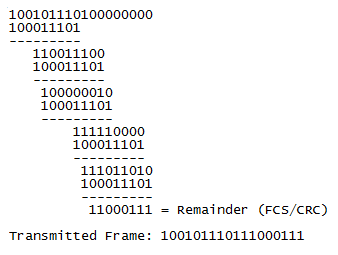
\includegraphics{./images/Aufgabe8c-sender}\\
Unsere zu verschickende Nachricht ist jetzt $\rightarrow$ 100101110111000111\\\\
Jetzt schicken wir diese Nachricht an den Empfänger und dieser führt ebenfalls eine Polynomdivision durch. Er dividiert die erhaltene Nachricht mit dem Generatorpolynom. Wenn als Ergebnis nur Nullen rauskommen ist die Nachricht korekkt angekommen, andernfalls ist ein fehler in der empfangenen Nachricht.\\
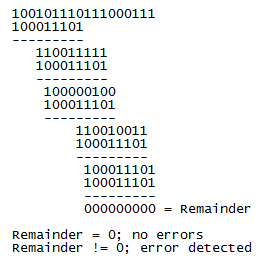
\includegraphics{./images/Aufgabe8c-empfaenger}\\

\end{document}
